% filepath: /Users/krzywdaja/Documents/quantum-gym/shadow_gym/paper/benchmark_explanation.tex
\documentclass[11pt, a4paper]{article}
\usepackage{amsmath, amssymb, amsthm}
\usepackage{graphicx}
\usepackage{hyperref}
\usepackage{xcolor}
\usepackage{tikz}
\usetikzlibrary{arrows.meta, positioning, shapes.geometric, fit, backgrounds, matrix}
\usepackage{listings}
\usepackage{booktabs}
\usepackage{geometry}
\usepackage{tcolorbox}
\usepackage{mdframed}
\geometry{margin=2.5cm}

\definecolor{codeblue}{RGB}{52, 152, 219}
\definecolor{codegray}{RGB}{149, 165, 166}
\definecolor{codegreen}{RGB}{46, 204, 113}
\definecolor{codered}{RGB}{231, 76, 60}
\definecolor{codeorange}{RGB}{230, 126, 34}
\definecolor{codepurple}{RGB}{155, 89, 182}
\definecolor{lightyellow}{RGB}{255, 249, 219}
\definecolor{lightblue}{RGB}{235, 245, 255}
\definecolor{lightgreen}{RGB}{235, 255, 240}

\tcbuselibrary{skins, breakable}

% Analogy box
\newtcolorbox{analogybox}[1]{
  colback=lightyellow,
  colframe=codeorange,
  fonttitle=\bfseries,
  title=Analogy: #1,
  breakable
}

% Key idea box
\newtcolorbox{keybox}[1]{
  colback=lightblue,
  colframe=codeblue,
  fonttitle=\bfseries,
  title=Key Idea: #1,
  breakable
}

% Intuition box
\newtcolorbox{intuitionbox}[1]{
  colback=lightgreen,
  colframe=codegreen!70!black,
  fonttitle=\bfseries,
  title=Intuition: #1,
  breakable
}

\lstset{
  basicstyle=\ttfamily\small,
  keywordstyle=\color{codeblue}\bfseries,
  commentstyle=\color{codegray},
  stringstyle=\color{codegreen},
  breaklines=true,
  frame=single,
  language=Python,
}

\title{
  \textbf{Neural World Models for Quantum State Tomography}\\
  \large From Classical Shadow Tomography to Active Inference:\\
  Theory, Intuition, and Implementation
}
\author{quantum-gym}
\date{\today}

\begin{document}
\maketitle
\tableofcontents
\newpage

% =============================================================================
\section{Overview}
% =============================================================================

The \texttt{benchmark\_world\_models.py} script benchmarks three neural
\emph{world models} against a random baseline in an \textbf{active learning
loop} for quantum state tomography. The central question is:

\begin{center}
\textit{Given a fixed budget of quantum measurements (shots), which model
recovers the stabilizer structure of a cluster state fastest?}
\end{center}

The script sits at the intersection of three ideas:
\begin{enumerate}
  \item \textbf{Classical Shadow Tomography} — efficient state estimation from
        random Pauli measurements.
  \item \textbf{Active Inference} — choosing \emph{which} measurements to
        perform next, guided by Expected Free Energy (EFE).
  \item \textbf{Neural World Models} — parameterised models
        (NQS, VAE, MADE-VAE) that learn a compressed representation of the
        quantum state from measurement data.
\end{enumerate}

% =============================================================================
\section{Background: Classical Shadow Tomography}
% =============================================================================

\subsection{The Shadow Channel}

Given an $n$-qubit state $\rho$, perform a random unitary $U$ drawn from a
fixed ensemble $\mathcal{E}$ (e.g.\ tensor products of single-qubit Clifford
unitaries), measure in the computational basis, and record outcome
$\hat{b} \in \{0,1\}^n$. The \emph{classical shadow} is:

\begin{equation}
  \hat{\sigma} = \mathcal{M}^{-1}\!\left(U^\dagger |\hat{b}\rangle\langle\hat{b}| U\right),
\end{equation}

where $\mathcal{M}$ is the \emph{shadow channel}:

\begin{equation}
  \mathcal{M}(\rho) = \mathbb{E}_{U \sim \mathcal{E}}\!\left[
    U^\dagger \!\left(\sum_b \langle b|U\rho U^\dagger|b\rangle\, |b\rangle\langle b|\right)\! U
  \right].
\end{equation}

For the random single-qubit Pauli ensemble (each qubit independently
measured in $X$, $Y$, or $Z$ with equal probability $\tfrac{1}{3}$), the
channel inverts as:

\begin{equation}
  \mathcal{M}^{-1}(\cdot) = \bigotimes_{i=1}^{n} (3\, (\cdot) - \mathbf{I}).
\end{equation}

\subsection{Pauli Estimators}

The unbiased estimator of a Pauli observable
$P = \bigotimes_{i=1}^n P_i$, $P_i \in \{I, X, Y, Z\}$, from a single
shadow $(b, s)$ is:

\begin{equation}
  \hat{v}_P(b, s) =
  \begin{cases}
    \prod_{i:\, P_i \neq I} 3\, s_i & \text{if } P_i = b_i \text{ for all } i \text{ where } P_i \neq I,\\
    0 & \text{otherwise.}
  \end{cases}
\end{equation}

\subsection{Stabilizer Fidelity}

\begin{equation}
  \boxed{F_{\mathrm{stab}}(\rho_{\mathrm{model}}) =
  \frac{1}{n}\sum_{i=1}^{n} \frac{1 + \langle K_i \rangle_{\mathrm{model}}}{2}
  \;\in [0, 1].}
\end{equation}

% =============================================================================
\section{What is an Autoregressive Model?}
% =============================================================================

\begin{analogybox}{Writing a sentence word by word}
Imagine writing the sentence \textit{``The cat sat on the mat''} one word at
a time. When you write \textit{``sat''}, you already know \textit{``The cat''}
came before. An autoregressive model does exactly this: it predicts each
token (or bit) \emph{conditioned on everything it has already generated}.
It never looks ahead — only backward.
\end{analogybox}

\subsection{The Chain Rule of Probability}

Any joint probability distribution over $n$ variables can be \emph{exactly}
factored using the chain rule:

\begin{equation}
  p(s_1, s_2, \ldots, s_n) =
  p(s_1)\cdot
  p(s_2 \mid s_1)\cdot
  p(s_3 \mid s_1, s_2)\cdots
  p(s_n \mid s_1, \ldots, s_{n-1}).
\end{equation}

This is not an approximation — it is always true. The question is
\emph{how} to parameterise each conditional. An autoregressive model uses a
neural network for each conditional.

\subsection{A Simple 3-Qubit Example}

Suppose we measure 3 qubits in basis $b = (X, Z, Y)$ and get outcome
$s = (+1, -1, +1)$.

An autoregressive model computes:

\begin{align}
  p(s_1 = +1 \mid b)                     &= \sigma(f_1(b)),\\
  p(s_2 = -1 \mid s_1 = +1,\; b)        &= \sigma(f_2(s_1, b)),\\
  p(s_3 = +1 \mid s_1 = +1, s_2 = -1,\; b) &= \sigma(f_3(s_1, s_2, b)),
\end{align}

where $\sigma$ is the sigmoid function and $f_i$ are small neural networks.
The joint probability is then:

\begin{equation}
  p(s \mid b) = p(s_1 \mid b)\cdot p(s_2 \mid s_1, b)\cdot p(s_3 \mid s_1, s_2, b).
\end{equation}

\vspace{0.5em}

\begin{center}
\begin{tikzpicture}[
  node distance=1.6cm,
  qubit/.style={circle, draw, thick, minimum size=0.9cm,
                font=\small\bfseries, fill=codeblue!20},
  net/.style={rectangle, rounded corners=3pt, draw, thick,
              minimum width=2.2cm, minimum height=0.7cm,
              fill=codeorange!20, font=\small},
  prob/.style={rectangle, rounded corners=3pt, draw, thick,
               minimum width=2.2cm, minimum height=0.7cm,
               fill=codegreen!20, font=\small},
  arrow/.style={-{Stealth[length=5pt]}, thick},
  dasharrow/.style={-{Stealth[length=5pt]}, thick, dashed, gray}
]

% Qubit nodes
\node[qubit] (q1) {$s_1$};
\node[qubit, right=2.4cm of q1] (q2) {$s_2$};
\node[qubit, right=2.4cm of q2] (q3) {$s_3$};

% Basis input
\node[above=0.6cm of q1, font=\small, text=codepurple] (b1) {$b_1=X$};
\node[above=0.6cm of q2, font=\small, text=codepurple] (b2) {$b_2=Z$};
\node[above=0.6cm of q3, font=\small, text=codepurple] (b3) {$b_3=Y$};

\draw[arrow, codepurple] (b1) -- (q1);
\draw[arrow, codepurple] (b2) -- (q2);
\draw[arrow, codepurple] (b3) -- (q3);

% Network boxes below
\node[net, below=0.8cm of q1] (n1) {$f_1(b)$};
\node[net, below=0.8cm of q2] (n2) {$f_2(s_1, b)$};
\node[net, below=0.8cm of q3] (n3) {$f_3(s_1, s_2, b)$};

% Probability outputs
\node[prob, below=0.5cm of n1] (p1) {$p(s_1|b)$};
\node[prob, below=0.5cm of n2] (p2) {$p(s_2|s_1,b)$};
\node[prob, below=0.5cm of n3] (p3) {$p(s_3|s_1,s_2,b)$};

% Arrows net->prob
\draw[arrow] (n1) -- (p1);
\draw[arrow] (n2) -- (p2);
\draw[arrow] (n3) -- (p3);

% Arrows qubit->net
\draw[arrow] (q1) -- (n1);
\draw[arrow] (q2) -- (n2);
\draw[arrow] (q3) -- (n3);

% Autoregressive arrows (s1 -> n2, s1+s2 -> n3)
\draw[dasharrow] (q1) to[out=-30, in=150] (n2);
\draw[dasharrow] (q1) to[out=-20, in=160] (n3);
\draw[dasharrow] (q2) to[out=-30, in=130] (n3);

% Labels on dashed arrows
\node[font=\tiny, text=gray, below=0.1cm] at ($(q1)!0.5!(n2)+(0,-0.3)$)
  {context};

\end{tikzpicture}
\end{center}

\vspace{0.5em}

\begin{keybox}{The autoregressive property}
Each network $f_i$ only receives \emph{past} outcomes $s_1, \ldots, s_{i-1}$
as context. This is the \textbf{autoregressive property}: no information from
the future leaks into the prediction. It guarantees a valid normalised
probability distribution without any extra constraints.
\end{keybox}

% =============================================================================
\section{Is Autoregressive the Same as an RNN?}
% =============================================================================

\begin{intuitionbox}{Short answer}
An RNN is \emph{one way} to implement an autoregressive model, but not the
only way. The autoregressive property is a \emph{structural constraint on
information flow}, not a specific architecture.
\end{intuitionbox}

\subsection{Three Ways to be Autoregressive}

\begin{center}
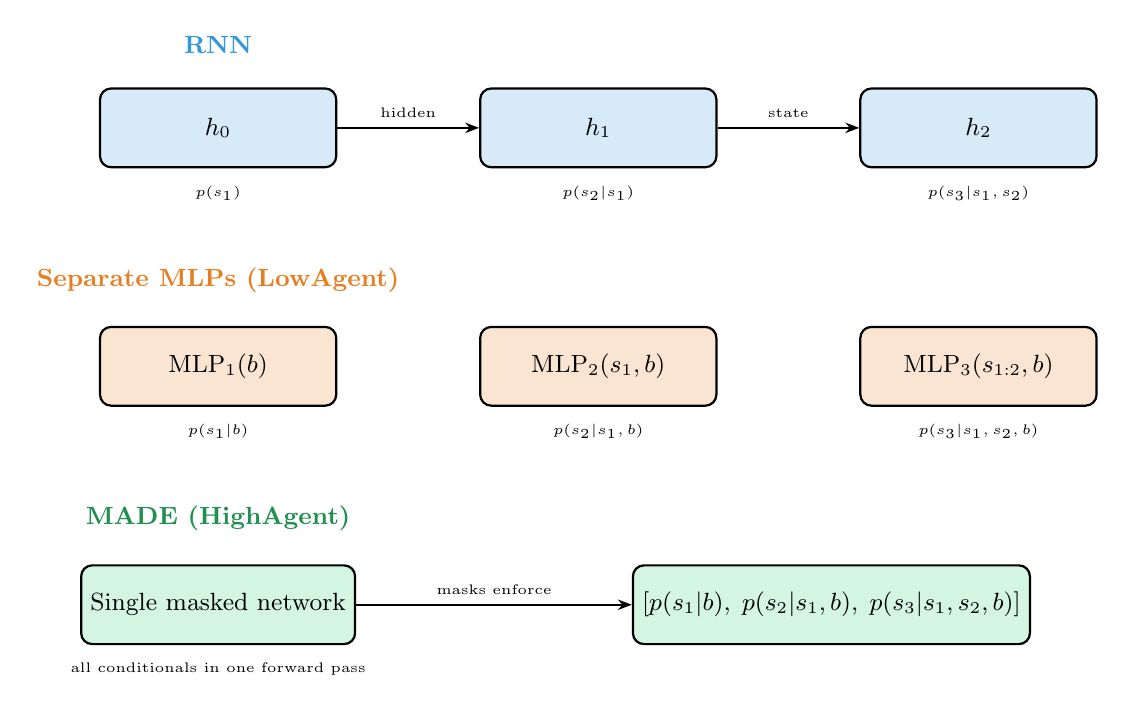
\begin{tikzpicture}[
  box/.style={rectangle, rounded corners=4pt, draw, thick,
              minimum width=3cm, minimum height=1cm,
              text centered, font=\small},
  arrow/.style={-{Stealth[length=5pt]}, thick},
  node distance=1.4cm and 1.8cm
]

% RNN column
\node[box, fill=codeblue!20]   (rnn1) {$h_0$};
\node[box, fill=codeblue!20, right=of rnn1] (rnn2) {$h_1$};
\node[box, fill=codeblue!20, right=of rnn2] (rnn3) {$h_2$};
\node[above=0.3cm of rnn1, font=\small\bfseries, text=codeblue] {RNN};
\draw[arrow] (rnn1) -- node[above, font=\tiny]{hidden} (rnn2);
\draw[arrow] (rnn2) -- node[above, font=\tiny]{state} (rnn3);
\node[below=0.1cm of rnn1, font=\tiny]{$p(s_1)$};
\node[below=0.1cm of rnn2, font=\tiny]{$p(s_2|s_1)$};
\node[below=0.1cm of rnn3, font=\tiny]{$p(s_3|s_1,s_2)$};

% MLP column
\node[box, fill=codeorange!20, below=2cm of rnn1] (mlp1) {MLP$_1(b)$};
\node[box, fill=codeorange!20, right=of mlp1]     (mlp2) {MLP$_2(s_1,b)$};
\node[box, fill=codeorange!20, right=of mlp2]     (mlp3) {MLP$_3(s_{1:2},b)$};
\node[above=0.3cm of mlp1, font=\small\bfseries, text=codeorange] {Separate MLPs (LowAgent)};
\node[below=0.1cm of mlp1, font=\tiny]{$p(s_1|b)$};
\node[below=0.1cm of mlp2, font=\tiny]{$p(s_2|s_1,b)$};
\node[below=0.1cm of mlp3, font=\tiny]{$p(s_3|s_1,s_2,b)$};

% MADE column
\node[box, fill=codegreen!20, below=2cm of mlp1] (made) {Single masked network};
\node[above=0.3cm of made, font=\small\bfseries, text=codegreen!70!black]
  {MADE (HighAgent)};
\node[below=0.1cm of made, font=\tiny]
  {all conditionals in one forward pass};
\node[box, fill=codegreen!20, right=3.5cm of made] (madeout)
  {$[p(s_1|b),\; p(s_2|s_1,b),\; p(s_3|s_1,s_2,b)]$};
\draw[arrow] (made) -- node[above, font=\tiny]{masks enforce} (madeout);

\end{tikzpicture}
\end{center}

\subsection{RNN as an Autoregressive Model}

An RNN processes sequence left-to-right. At step $i$:

\begin{align}
  h_i &= \tanh(W_h h_{i-1} + W_x s_{i-1} + W_b b_i + c_h),\\
  p(s_i \mid s_{<i}, b) &= \sigma(W_o h_i + c_o).
\end{align}

The hidden state $h_i$ compresses all past information into a fixed-size
vector. This is exactly the autoregressive property, implemented via
\emph{recurrence}.

\begin{analogybox}{RNN as a reader}
Think of an RNN as a person reading a book. After reading each word, they
update their ``understanding'' (hidden state $h_i$). Their prediction of the
next word depends only on their current understanding, not on re-reading the
whole book from scratch.
\end{analogybox}

\subsection{LowAgent: Separate MLPs (Simpler, Faster)}

\texttt{LowAgent} avoids recurrence entirely. It uses $n$ \emph{separate}
small MLPs, one per qubit:

\begin{equation}
  p_\theta(s_i \mid s_{<i}, b) = \sigma\!\left(\mathrm{MLP}_i([s_1, \ldots, s_{i-1}, b_1, \ldots, b_n])\right).
\end{equation}

The input to MLP$_i$ is simply the concatenation of all previous outcomes
and the full basis string.

\begin{center}
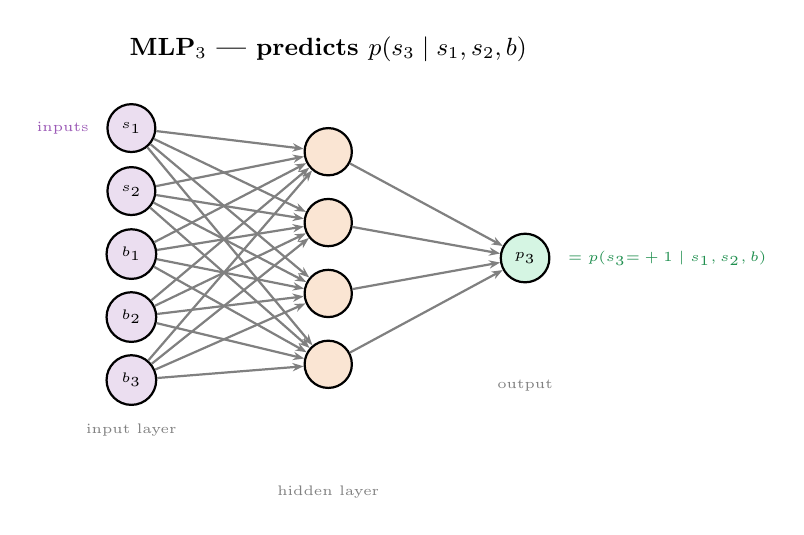
\begin{tikzpicture}[
  input/.style={circle, draw, thick, minimum size=0.6cm, font=\tiny,
                fill=codepurple!20},
  hidden/.style={circle, draw, thick, minimum size=0.6cm, font=\tiny,
                 fill=codeorange!20},
  output/.style={circle, draw, thick, minimum size=0.6cm, font=\tiny,
                 fill=codegreen!20},
  arrow/.style={-{Stealth[length=4pt]}, thick, gray},
  node distance=0.5cm
]

% MLP_3 example: predicts s_3 given s_1, s_2, b_1, b_2, b_3
\node[font=\small\bfseries] at (0, 3.5) {MLP$_3$ — predicts $p(s_3 \mid s_1, s_2, b)$};

% Input layer
\node[input] (i1) at (-2.5, 2.5) {$s_1$};
\node[input] (i2) at (-2.5, 1.7) {$s_2$};
\node[input] (i3) at (-2.5, 0.9) {$b_1$};
\node[input] (i4) at (-2.5, 0.1) {$b_2$};
\node[input] (i5) at (-2.5,-0.7) {$b_3$};
\node[left=0.1cm of i1, font=\tiny, text=codepurple] {inputs};

% Hidden layer
\node[hidden] (h1) at (0, 2.2) {};
\node[hidden] (h2) at (0, 1.3) {};
\node[hidden] (h3) at (0, 0.4) {};
\node[hidden] (h4) at (0,-0.5) {};

% Output
\node[output] (o1) at (2.5, 0.85) {$p_3$};
\node[right=0.1cm of o1, font=\tiny, text=codegreen!70!black]
  {$= p(s_3{=}+1 \mid s_1,s_2,b)$};

% Arrows input->hidden
\foreach \i in {i1,i2,i3,i4,i5}
  \foreach \h in {h1,h2,h3,h4}
    \draw[arrow] (\i) -- (\h);

% Arrows hidden->output
\foreach \h in {h1,h2,h3,h4}
  \draw[arrow] (\h) -- (o1);

% Layer labels
\node[below=0.1cm of i5, font=\tiny, text=gray] {input layer};
\node[below=1.1cm of h4, font=\tiny, text=gray] {hidden layer};
\node[below=1.1cm of o1, font=\tiny, text=gray] {output};

\end{tikzpicture}
\end{center}

\begin{intuitionbox}{Why not use an RNN here?}
For 6--11 qubits, the sequences are very short. The benefit of weight-sharing
across positions (the main advantage of RNNs) is minimal. Separate MLPs are
simpler to train, easier to parallelize, and avoid vanishing gradient
problems. The \texttt{LowAgent} trades model capacity for training speed —
appropriate when data (shots) are scarce.
\end{intuitionbox}

% =============================================================================
\section{What is a Neural Quantum State (NQS)?}
% =============================================================================

\begin{analogybox}{NQS as a compressed photograph}
A quantum state on $n$ qubits lives in a $2^n$-dimensional Hilbert space.
Storing the full state vector for $n=20$ would require $2^{20} \approx 10^6$
complex numbers. An NQS is like a compressed photograph: instead of storing
every pixel, you store the parameters of a neural network that can
\emph{regenerate} any pixel on demand. The network is far smaller than the
full state but can approximate it well.
\end{analogybox}

Formally, an NQS parameterises the wave function amplitude directly:

\begin{equation}
  \psi_\theta(s) = \langle s | \psi \rangle
  \;\approx\;
  \mathrm{NeuralNet}_\theta(s),
\end{equation}

or, in the \texttt{LowAgent} case, the \emph{conditional Born probability}
of measurement outcomes:

\begin{equation}
  p_\theta(s \mid b) \approx |\langle s_b | \psi \rangle|^2,
\end{equation}

where $|s_b\rangle$ is the basis-rotated computational state. The neural
network learns this distribution from data — no explicit wave function is
stored.

\subsection{Why Autoregressive?}

For the model to define a valid probability distribution, probabilities must
sum to 1:

\begin{equation}
  \sum_{s \in \{-1,+1\}^n} p_\theta(s \mid b) = 1.
\end{equation}

The autoregressive factorisation guarantees this \emph{automatically}:
each conditional $p(s_i \mid s_{<i}, b)$ is a Bernoulli distribution
(a single sigmoid), which trivially sums to 1. No normalisation constant
needs to be computed, avoiding the intractable partition function that plagues
energy-based models.

\begin{center}
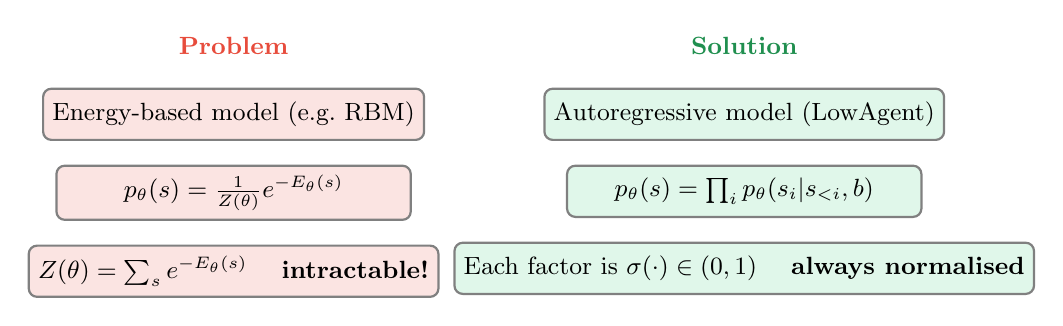
\begin{tikzpicture}[
  node distance=0.8cm,
  box/.style={rectangle, rounded corners=3pt, draw=gray, thick,
              minimum width=4.5cm, minimum height=0.65cm,
              text centered, font=\small}
]
\node[box, fill=codered!15]    (e1) {Energy-based model (e.g.\ RBM)};
\node[box, fill=codered!15, below=0.3cm of e1] (e2)
  {$p_\theta(s) = \frac{1}{Z(\theta)}e^{-E_\theta(s)}$};
\node[box, fill=codered!15, below=0.3cm of e2] (e3)
  {$Z(\theta) = \sum_s e^{-E_\theta(s)}$ \quad \textbf{intractable!}};

\node[box, fill=codegreen!15, right=1.5cm of e1] (a1)
  {Autoregressive model (LowAgent)};
\node[box, fill=codegreen!15, below=0.3cm of a1] (a2)
  {$p_\theta(s) = \prod_i p_\theta(s_i | s_{<i}, b)$};
\node[box, fill=codegreen!15, below=0.3cm of a2] (a3)
  {Each factor is $\sigma(\cdot) \in (0,1)$ \quad \textbf{always normalised}};

\node[above=0.3cm of e1, font=\small\bfseries, text=codered] {Problem};
\node[above=0.3cm of a1, font=\small\bfseries, text=codegreen!70!black] {Solution};
\end{tikzpicture}
\end{center}

% =============================================================================
\section{MidAgent: Variational Autoencoder (VAE)}
% =============================================================================

\begin{analogybox}{VAE as a sketch artist}
Imagine an artist who, upon seeing a measurement outcome $s$, first sketches
a compressed ``essence'' of the state (the latent variable $z$), then
reconstructs the full picture from that sketch. The VAE does this
mathematically: an \emph{encoder} compresses $(s, b) \to z$, a
\emph{decoder} reconstructs $s$ from $z$ autoregressively.
\end{analogybox}

The VAE introduces a latent variable $z \in \mathbb{R}^d$ to capture
global correlations:

\begin{center}
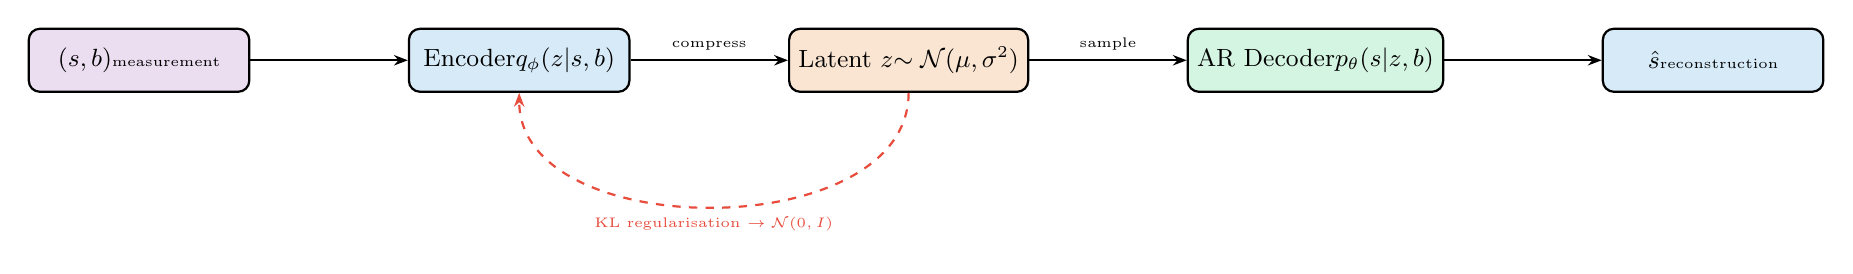
\begin{tikzpicture}[
  box/.style={rectangle, rounded corners=4pt, draw, thick,
              minimum width=2.8cm, minimum height=0.8cm,
              text centered, font=\small},
  arrow/.style={-{Stealth[length=5pt]}, thick},
  node distance=1.2cm and 2cm
]

\node[box, fill=codepurple!20] (input) {$(s, b)$\\{\tiny measurement}};
\node[box, fill=codeblue!20, right=of input] (enc) {Encoder\\$q_\phi(z|s,b)$};
\node[box, fill=codeorange!20, right=of enc] (latent) {Latent $z$\\$\sim \mathcal{N}(\mu,\sigma^2)$};
\node[box, fill=codegreen!20, right=of latent] (dec) {AR Decoder\\$p_\theta(s|z,b)$};
\node[box, fill=codeblue!20, right=of dec] (out) {$\hat{s}$\\{\tiny reconstruction}};

\draw[arrow] (input) -- (enc);
\draw[arrow] (enc)   -- node[above, font=\tiny]{compress} (latent);
\draw[arrow] (latent)-- node[above, font=\tiny]{sample} (dec);
\draw[arrow] (dec)   -- (out);

% KL arrow
\draw[arrow, codered, dashed] (latent) to[out=-90, in=-90]
  node[below, font=\tiny, text=codered]{KL regularisation $\to \mathcal{N}(0,I)$}
  (enc);

\end{tikzpicture}
\end{center}

Training objective (ELBO):

\begin{equation}
  \mathcal{L}_{\mathrm{VAE}} =
  \underbrace{\mathbb{E}_{q_\phi(z|s,b)}[\ln p_\theta(s \mid z, b)]}_{\text{reconstruction}}
  - \beta\,\underbrace{D_{\mathrm{KL}}(q_\phi(z \mid s, b) \,\|\, \mathcal{N}(0, I))}_{\text{regularisation}}.
\end{equation}

The latent $z$ captures global features of the quantum state that correlate
across all qubits — something the independent MLPs of \texttt{LowAgent}
cannot represent.

% =============================================================================
\section{HighAgent: MADE — One Network, All Conditionals}
% =============================================================================

\begin{analogybox}{MADE as a parallel factory}
In \texttt{LowAgent}, each conditional $p(s_i | s_{<i}, b)$ is computed by a
\emph{separate} MLP — like having $n$ separate workers each doing one job.
MADE uses a \emph{single} network but applies binary masks to the weights,
ensuring that the output for qubit $i$ depends only on inputs $s_1, \ldots,
s_{i-1}$. It is like one worker with a blindfold that blocks them from seeing
``future'' inputs.
\end{analogybox}

Each weight matrix $W^{(l)}$ is elementwise-multiplied by a binary mask:

\begin{equation}
  \tilde{W}^{(l)}_{ij} = W^{(l)}_{ij} \odot M^{(l)}_{ij},
  \qquad
  M^{(l)}_{ij} = \mathbf{1}\!\left[m^{(l)}(i) \geq m^{(l-1)}(j)\right],
\end{equation}

where $m^{(l)}(i) \in \{1, \ldots, n\}$ is the \emph{order} assigned to
unit $i$ in layer $l$.

\begin{center}
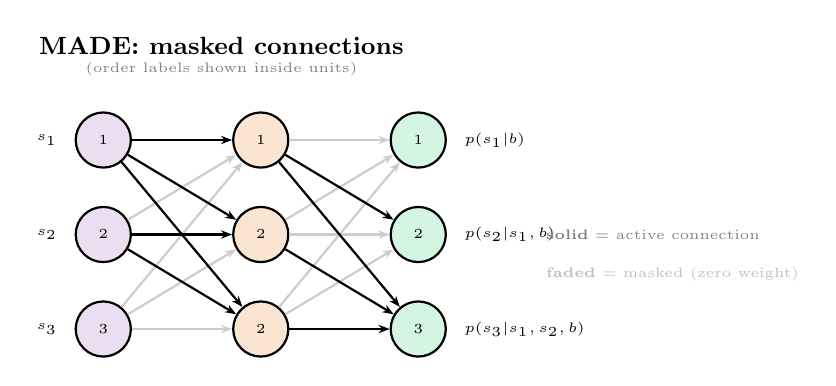
\begin{tikzpicture}[
  unit/.style={circle, draw, thick, minimum size=0.7cm, font=\tiny},
  arrow/.style={-{Stealth[length=4pt]}, thick},
  garrow/.style={-{Stealth[length=4pt]}, thick, gray!40},
  node distance=0.4cm
]

\node[font=\small\bfseries] at (1.5, 4.2) {MADE: masked connections};
\node[font=\tiny, text=gray] at (1.5, 3.9) {(order labels shown inside units)};

% Input layer (order 1,2,3)
\node[unit, fill=codepurple!20] (x1) at (0, 3)   {1};
\node[unit, fill=codepurple!20] (x2) at (0, 1.8) {2};
\node[unit, fill=codepurple!20] (x3) at (0, 0.6) {3};
\node[left=0.1cm of x1, font=\tiny]{$s_1$};
\node[left=0.1cm of x2, font=\tiny]{$s_2$};
\node[left=0.1cm of x3, font=\tiny]{$s_3$};

% Hidden layer (order 1,2,2)
\node[unit, fill=codeorange!20] (h1) at (2, 3)   {1};
\node[unit, fill=codeorange!20] (h2) at (2, 1.8) {2};
\node[unit, fill=codeorange!20] (h3) at (2, 0.6) {2};

% Output layer (order 1,2,3) — predicts next token
\node[unit, fill=codegreen!20] (o1) at (4, 3)   {1};
\node[unit, fill=codegreen!20] (o2) at (4, 1.8) {2};
\node[unit, fill=codegreen!20] (o3) at (4, 0.6) {3};
\node[right=0.1cm of o1, font=\tiny]{$p(s_1|b)$};
\node[right=0.1cm of o2, font=\tiny]{$p(s_2|s_1,b)$};
\node[right=0.1cm of o3, font=\tiny]{$p(s_3|s_1,s_2,b)$};

% Input -> Hidden: only if m_h >= m_x
% h1(1): only x1(1) — no, rule is m_h >= m_x means 1>=1 yes, 1>=2 no, 1>=3 no
\draw[arrow] (x1) -- (h1); % 1>=1
\draw[garrow] (x2) -- (h1); % 1>=2 no
\draw[garrow] (x3) -- (h1); % 1>=3 no

% h2(2): x1(1) yes, x2(2) yes, x3(3) no
\draw[arrow] (x1) -- (h2);
\draw[arrow] (x2) -- (h2);
\draw[garrow] (x3) -- (h2);

% h3(2): same as h2
\draw[arrow] (x1) -- (h3);
\draw[arrow] (x2) -- (h3);
\draw[garrow] (x3) -- (h3);

% Hidden -> Output: m_o > m_h (strict for output)
% o1(1): h1(1) no (not strict), h2(2) no, h3(2) no
\draw[garrow] (h1) -- (o1);
\draw[garrow] (h2) -- (o1);
\draw[garrow] (h3) -- (o1);

% o2(2): h1(1) yes, h2(2) no, h3(2) no
\draw[arrow] (h1) -- (o2);
\draw[garrow] (h2) -- (o2);
\draw[garrow] (h3) -- (o2);

% o3(3): h1(1) yes, h2(2) yes, h3(2) yes
\draw[arrow] (h1) -- (o3);
\draw[arrow] (h2) -- (o3);
\draw[arrow] (h3) -- (o3);

% Legend
\node[right=0.5cm of o1, font=\tiny, text=gray] at (5, 1.8)
  {\textbf{solid} = active connection};
\node[right=0.5cm of o2, font=\tiny, text=gray!50] at (5, 1.3)
  {\textbf{faded} = masked (zero weight)};

\end{tikzpicture}
\end{center}

The key advantage: \textbf{all $n$ conditionals are computed in a single
forward pass}, making \texttt{HighAgent} faster to evaluate than
$n$ separate MLP calls during EFE scoring.

% =============================================================================
\section{Comparison of the Three Agents}
% =============================================================================

\begin{table}[h]
\centering
\renewcommand{\arraystretch}{1.4}
\begin{tabular}{lllll}
\toprule
\textbf{Agent} & \textbf{Architecture} & \textbf{Like an RNN?} &
\textbf{Latent space?} & \textbf{Forward passes} \\
\midrule
LowAgent  & $n$ separate MLPs     & No  & No  & $n$ (one per qubit)   \\
MidAgent  & AR-VAE                & No  & Yes & $n + $ encoder        \\
HighAgent & MADE-VAE              & No  & Yes & 1 (masks do the work) \\
Random    & LowAgent (no EFE)     & No  & No  & $n$                   \\
\bottomrule
\end{tabular}
\caption{Architectural comparison of the four benchmark agents.}
\end{table}

\begin{keybox}{None of them are RNNs}
All three models implement the autoregressive factorisation
\emph{without recurrence}. This avoids vanishing gradients, allows
full parallelism during training, and is well-suited to the short
sequences ($n \leq 20$) typical of quantum tomography experiments.
\end{keybox}

% =============================================================================
\section{The Active Learning Pipeline}
% =============================================================================

\begin{center}
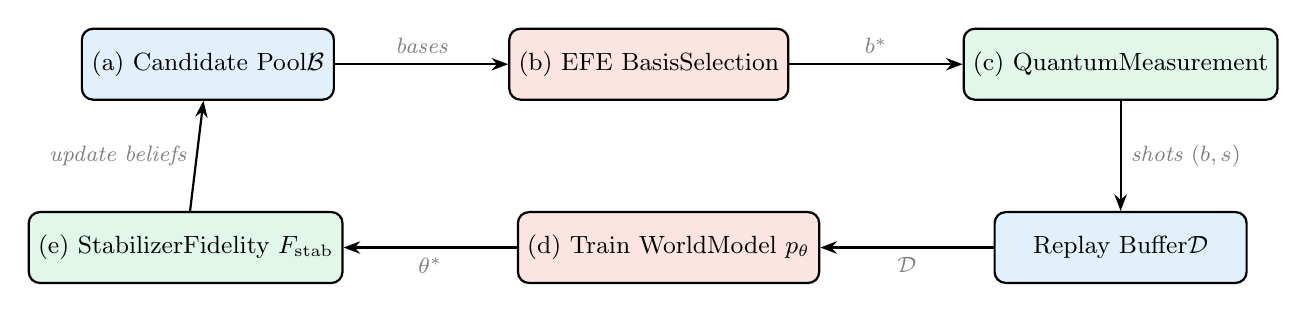
\begin{tikzpicture}[
  node distance=1.4cm and 2.2cm,
  box/.style={rectangle, rounded corners=4pt, draw, thick,
              minimum width=3.2cm, minimum height=0.9cm,
              text centered, font=\small},
  arrow/.style={-{Stealth[length=6pt]}, thick},
  label/.style={font=\footnotesize\itshape, text=gray}
]
\node[box, fill=codeblue!15]   (pool)   {(a) Candidate Pool\\$\mathcal{B}$};
\node[box, fill=codered!15,    right=of pool]  (select) {(b) EFE Basis\\Selection};
\node[box, fill=codegreen!15,  right=of select](measure){(c) Quantum\\Measurement};
\node[box, fill=codeblue!15,   below=of measure](buffer) {Replay Buffer\\$\mathcal{D}$};
\node[box, fill=codered!15,    left=of buffer] (train)  {(d) Train World\\Model $p_\theta$};
\node[box, fill=codegreen!15,  left=of train]  (eval)   {(e) Stabilizer\\Fidelity $F_{\rm stab}$};

\draw[arrow] (pool)    -- node[above, label]{bases} (select);
\draw[arrow] (select)  -- node[above, label]{$b^*$} (measure);
\draw[arrow] (measure) -- node[right, label]{shots $(b,s)$} (buffer);
\draw[arrow] (buffer)  -- node[below, label]{$\mathcal{D}$} (train);
\draw[arrow] (train)   -- node[below, label]{$\theta^*$} (eval);
\draw[arrow] (eval)    -- node[left,  label]{update beliefs} (pool);
\end{tikzpicture}
\end{center}

% =============================================================================
\section{Relationship to Classical Shadow Tomography}
% =============================================================================

\begin{table}[h]
\centering
\renewcommand{\arraystretch}{1.3}
\begin{tabular}{lll}
\toprule
\textbf{Component} & \textbf{Classical Shadows} & \textbf{This Work} \\
\midrule
Basis selection     & Uniform random $\{X,Y,Z\}^n$ & EFE-adaptive \\
State representation& Empirical average $\hat{\rho}$ & Neural $p_\theta(s|b)$ \\
Channel inversion   & Explicit $\mathcal{M}^{-1}$   & Implicit (likelihood) \\
Observable estimation & Unbiased Pauli estimator & $\mathbb{E}_{p_\theta}[\hat{v}_{K_i}]$ \\
Sample complexity   & $\mathcal{O}(\log M / \epsilon^2)$ & Empirically lower \\
\bottomrule
\end{tabular}
\caption{Classical shadow tomography vs.\ neural active inference.}
\end{table}

The \texttt{RandomAgent} \emph{is} classical shadow tomography. The
\texttt{Low/Mid/HighAgent} add active inference on top, replacing the
uniform random policy with an EFE-driven policy that targets
stabilizer-relevant measurements.

% =============================================================================
\section{Summary}
% =============================================================================

\begin{enumerate}
  \item \textbf{Autoregressive models} decompose $p(s|b)$ using the chain
        rule. This is not unique to RNNs — it can be implemented with
        separate MLPs (LowAgent) or masked networks (HighAgent).
  \item \textbf{NQS} is the idea of using a neural network to represent a
        quantum state implicitly, avoiding exponential memory.
  \item \textbf{VAE} adds a latent space to capture global correlations
        across qubits, at the cost of a more complex training objective.
  \item \textbf{MADE} achieves the same autoregressive property as separate
        MLPs but in a single forward pass, via binary weight masks.
  \item \textbf{RandomAgent} is classical shadow tomography — the correct
        statistical baseline.
  \item \textbf{Active inference} replaces random basis selection with
        EFE-driven selection, targeting measurements that most reduce
        uncertainty about the stabilizers.
\end{enumerate}

\end{document}